\documentclass[12pt,a4paper]{article}

\usepackage[utf8]{inputenc}
\usepackage{graphicx}
\usepackage{tikz}
\usetikzlibrary{shapes.geometric, arrows.meta, positioning, calc}
\usepackage{hyperref}
\usepackage{geometry}
\geometry{a4paper, margin=1in}
\usepackage{setspace}
\onehalfspacing

\title{\textbf{Romer Calypso Motor Driver Main Board}\\ \Large Technical Whitepaper}
\author{}
\date{}

\begin{document}
\maketitle

\begin{abstract}
This whitepaper details the design and architecture of the Romer Calypso Motor Driver Main Board. Acting as the critical interface between higher-level command systems and physical actuators, the system leverages an Arduino Uno R3 to safely and efficiently control the vessel's engines. This document outlines the hardware architecture, the communication protocol rationale, and the crucial safety precautions necessary for operation in a marine environment.
\end{abstract}

\section{System Architecture}
The core philosophy of the Romer Calypso Motor Driver system is to maintain a robust, decoupled interface between the high-level decision-making software (the "Master") and the physical hardware. The code living on the Arduino is solely responsible for translating received commands into safe, regulated power delivery to the engines, irrespective of the specific power source, provided it meets the hardware ratings.

\subsection{Hardware Components}
The central processing unit for this subsystem is an \textbf{Arduino Uno R3}. It serves as the bridge between the master control interface and the Electronic Speed Controllers (ESCs).

\begin{figure}[htpb]
    \centering
    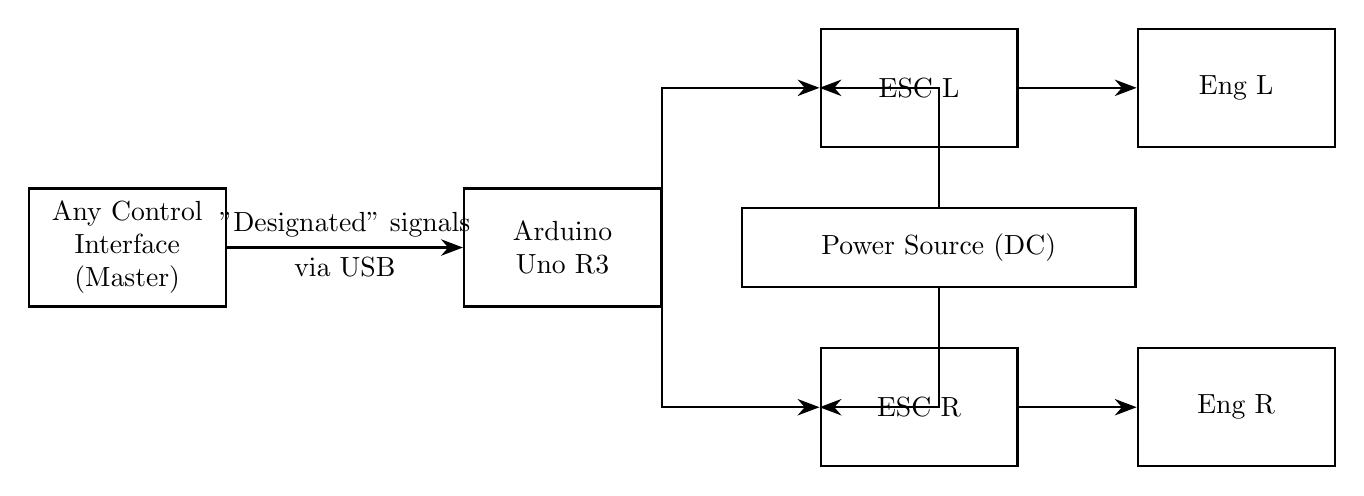
\begin{tikzpicture}[
        node distance=1.5cm and 2cm,
        box/.style={rectangle, draw=black, thick, minimum width=2.5cm, minimum height=1.5cm, align=center},
        arrow/.style={-{Stealth[scale=1.2]}, thick}
    ]

    % Nodes
    \node (master) [box] {Any Control\\Interface\\(Master)};
    \node (arduino) [box, right=3cm of master] {Arduino\\Uno R3};
    \node (escl) [box, above right=0.5cm and 2cm of arduino] {ESC L};
    \node (escr) [box, below right=0.5cm and 2cm of arduino] {ESC R};
    \node (engl) [box, right=1.5cm of escl] {Eng L};
    \node (engr) [box, right=1.5cm of escr] {Eng R};
    
    \node (power) [box, minimum width=5cm, minimum height=1cm, right=1cm of arduino, yshift=0cm] {Power Source (DC)};

    % Connections
    \draw [arrow] (master) -- node[above] {"Designated" signals} node[below] {via USB} (arduino);
    
    \draw [arrow] (arduino.east) |- (escl.west);
    \draw [arrow] (arduino.east) |- (escr.west);
    
    \draw [arrow] (escl) -- (engl);
    \draw [arrow] (escr) -- (engr);
    
    \draw [arrow] (power.north) |- (escl.west);
    \draw [arrow] (power.south) |- (escr.west);

    \end{tikzpicture}
    \caption{Romer Calypso Motor Driver Architecture}
    \label{fig:architecture}
\end{figure}

As shown in Figure \ref{fig:architecture}, the control interface communicates exclusively with the Arduino. The Arduino then dispatches control signals to the Left and Right ESCs. Simultaneously, a common DC Power Source provides the necessary current directly to the ESCs, which in turn drive the Left and Right Engines.

\section{Control Interface and Protocol}

\subsection{USB Serial Communication}
The communication link between the Master interface and the Arduino Uno R3 is established via \textbf{USB Serial (UART over USB)}. 

\textbf{Justification:} For a sea vehicle, reliability, simplicity, and ease of debugging are paramount. USB Serial offers a robust, universally supported protocol that is natively integrated into the Arduino Uno R3 architecture. It avoids the complexities and potential failure points of more intricate networking protocols (like Ethernet or CAN bus) for this specific short-range, point-to-point interface. A standard baud rate (e.g., 115200 bps) ensures sufficiently fast command transmission while maintaining high signal integrity, which is critical in environments prone to electromagnetic interference.

\section{Signal Protocol}
The Romer Calypso driver operates strictly as an actuator interface. The logic regarding environmental awareness (e.g., whether the vehicle is in water or on land) resides within the Master code. The Arduino expects explicit, pre-calculated commands.

\subsection{Motor Control Signals}
Control signals sent to the Arduino dictate three primary parameters: \textbf{(Direction [Forward/Reverse], \% Power, Duration)}.

\textbf{The Rationale for Duration:} Including a \textit{Duration} parameter in the command packet is a deliberate design choice aimed at optimizing system resources. Instead of the Master continuously polling and transmitting real-time adjustments (e.g., sending a "move forward" command every 10 milliseconds), it can issue a single command such as "Move Forward at 50\% Power for 2 seconds." 

This approach significantly reduces:
\begin{itemize}
    \item \textbf{Communication Overload:} Frees up the USB Serial bandwidth.
    \item \textbf{Calculation Overhead:} Allows the Master processor to enter low-power states or allocate CPU cycles to complex tasks (like navigation or image processing) without the burden of maintaining a real-time motor control loop.
\end{itemize}

\subsection{Emergency Stop (Cancel Command)}
Because commands are executed over a defined duration, a mechanism to preemptively halt operations is required. 
When a "Stop" or "Cancel Previous Command" signal is received, the Arduino immediately ceases driving the engines (dropping PWM signals to zero or neutral). This serves as a critical emergency brake, overriding any currently executing duration-based command.

\subsection{Telemetry Reporting}
To ensure the Master code can make informed decisions, the Arduino reports back critical hardware states:
\begin{enumerate}
    \item \textbf{Battery Voltage:} Reported back as an internal short-proof and power monitoring mechanism.
    \item \textbf{Dry/Wet Conditions:} The Arduino reports sensor data or state flags back to the Master. Note: The Arduino itself does not make decisions based on this data; it acts as a passthrough limiter. The Master analyzes this telemetry and dictates the appropriate power limits in its subsequent commands.
\end{enumerate}

\section{Precautions}
To prevent hardware damage, the following operational limits are strictly enforced:

\begin{itemize}
    \item \textbf{Maximum Voltage:} Under no circumstances should the DC Power Source supply a voltage higher than the maximum rating of the Electronic Speed Controllers (ESCs).
    \item \textbf{Dry Operation Power Limit:} When operating in a "dry" state (out of the water, lacking standard liquid cooling), the engines must \textbf{never run higher than 30\% power}. The Master code is responsible for recognizing the dry state and ensuring commands do not exceed this 30\% threshold, though the Arduino may also act as a secondary fail-safe limiter if instructed by the Master.
\end{itemize}

\end{document}
